%! TEX root = ../main.tex
\documentclass[main]{subfiles}

\begin{document}

\chapter{考察}
\section{重さ}
カーリング競技を行うにあたって,カーリングブラシを使用するほどカーリングブラシパッドの上のゴミが付着していくのでゴ
ミの分の質量が増加するように考えられるが,実際の結果では使用期間が長いほど質量は減っていた.これはカーリングブラシパッドの
表面繊維が摩耗して,繊維が擦り切れたことが原因だと考えられる.その上で,付着したゴミを考慮すると,どれほど摩耗
したか,正確な値を得ることはできなかった.しかし測定結果から付着して増えたゴミの質量よりもブラシパッドを使用
して摩耗して擦り切れた繊維の質量のほうが多いと言える.
\\

\section{表面繊維}
低倍率で比較したときに,使用期間が長いものほどゴミの付着量が多いことが分かった.高倍率で比較すると繊維が擦り切れて
細くなっているものがあった.繊維が軸方向に細分化しておりフィブリル化していた.
また,色が薄くなっていることや繊維と繊維の隙間が大きくなっていることは,繊維がフィブリル化
したことが原因であると考える.

実験結果からスイープ方向に垂直に並んでいる繊維がパッドの役割を果たしているものだと考えられる.未使用のものは繊維が
隙間なく並んでいるが,長期間使用したものは繊維と繊維の隙間が大きくなっている部分もあり,未使用のものと性能に違いが
出たとしたときの1つの要因として考えられる.

10~15投使用したものはFig.\ref{fig:labelX}とFig.\ref{fig:labelY}で摩耗具合が違った.サンプルBのほうが摩耗していた理由としては,使用する
際にブラシパッドのもつ向きが偏っていたことが考えられる.

\begin{figure}[htbp]
    \centering
    \begin{subfigure}[htbp]{0.3\linewidth}
        \centering
        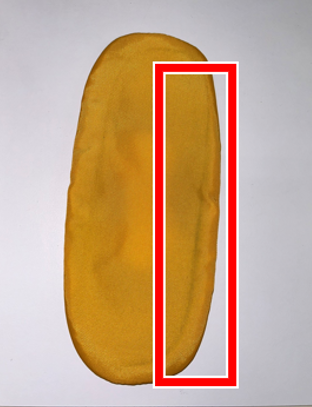
\includegraphics[keepaspectratio, width=0.8\linewidth, height=\linewidth]{figures/caring_brush_pad/10~15Akousatu.png}
        \caption{赤枠の汚れに偏りなし}
        \label{fig:labelX}
    \end{subfigure}
    \begin{subfigure}[htbp]{0.3\linewidth}
        \centering
        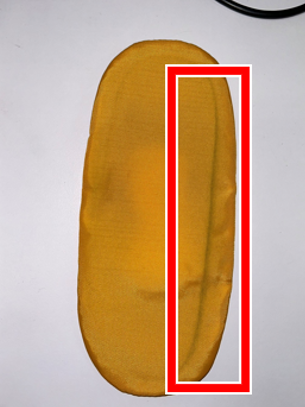
\includegraphics[keepaspectratio, width=0.8\linewidth, height=\linewidth]{figures/caring_brush_pad/10~15Bkousatu.png}
        \caption{赤枠の汚れに偏りあり}
        \label{fig:labelY}
    \end{subfigure}
    \caption{10~15投使用}
    \label{fig:label}
\end{figure}

Fig.\ref{fig:labelX}とFig.\ref{fig:labelY}を比較したときにFig.\ref{fig:labelX}の方がブラシパッドの右側が汚い
ことが分かる.このことから何投か使用した後にブラシパッドの倒す方向を逆にすることで左右に偏りなく使用することが
できる.
\\

\section{色の違い}
デジタルマイクロスコープを用いて撮影した表面繊維の色をRGB値で数値化し,それを基にHSVに変換した.HSVの値を見ると
彩度(S)の値が使用回数が多くなるほど小さくなっていった.このことから使用回数が多いほど色が段々と薄くなっている
ことが分かる.表面繊維の観察で考えたように,繊維がフィブリル化したことで全体の色素が薄くなったと考える.

\end{document}